In this section, 
we present the results of CNN on California and the three placebo states (Delware, Virginia, and Wyoming)
with two variations in the CNN architecture: (i) applying batch normalization and (ii) adding an additional convolution (with 16 outputs).

\subsection{Batch Normalization}



\begin{figure}[htbp]
    \centering
    \begin{subfigure}[b]{0.4\textwidth}
        \centering
        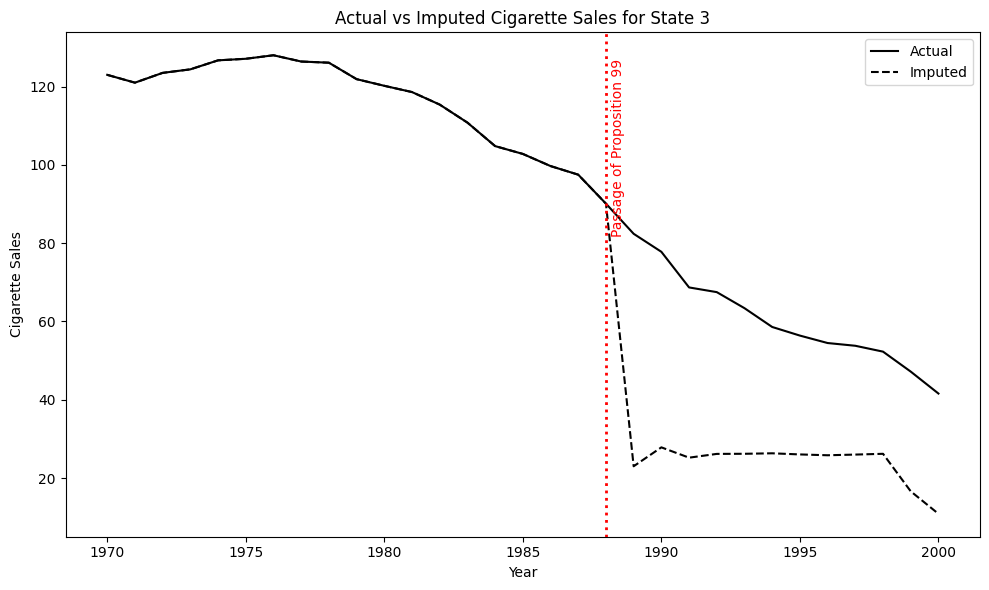
\includegraphics[width=\linewidth]{../figures/cnn_batch_norm-1.png}
        \caption{California}
        \label{fig:bn-cal}
    \end{subfigure}
    \hspace{1.5cm}
    \begin{subfigure}[b]{0.4\textwidth}
        \centering
        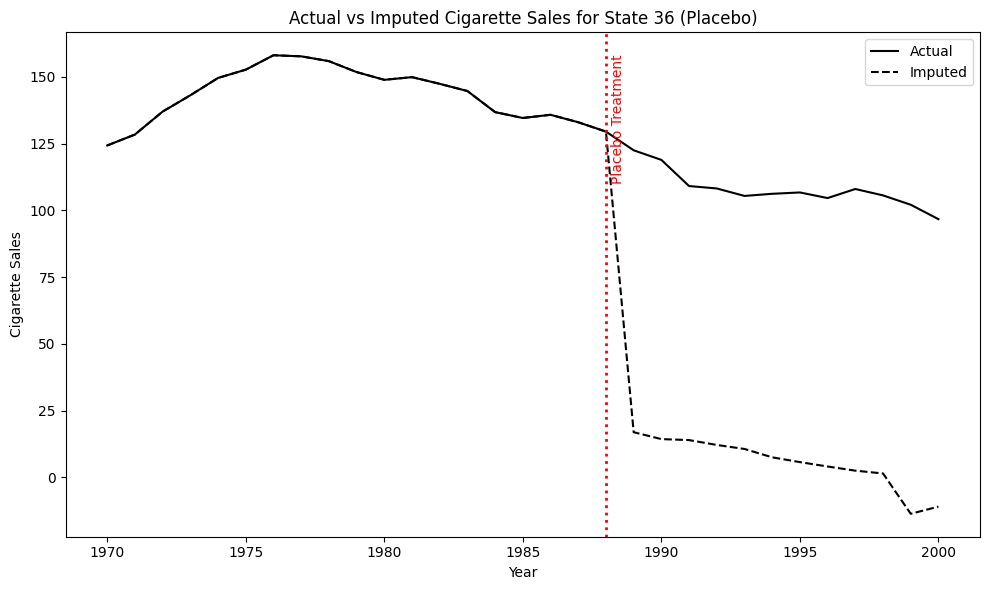
\includegraphics[width=\linewidth]{../figures/cnn_batch_norm-2.png}
        \caption{Delaware}
        \label{fig:bn-del}
    \end{subfigure}

    \vskip\baselineskip

    \begin{subfigure}[b]{0.4\textwidth}
        \centering
        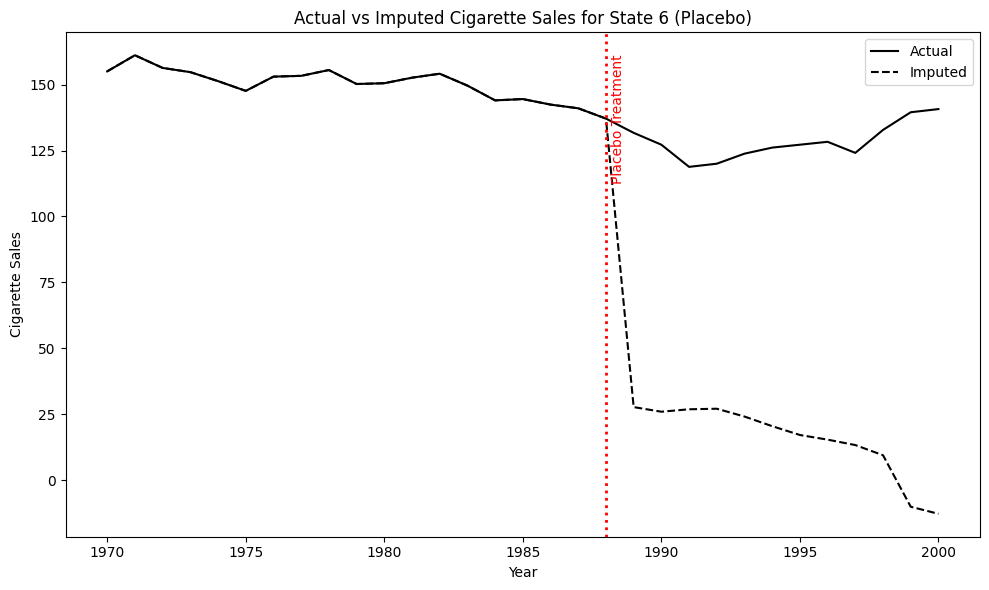
\includegraphics[width=\linewidth]{../figures/cnn_batch_norm-3.png}
        \caption{Virginia}
        \label{fig:bn-vir}
    \end{subfigure}
    \hspace{1.5cm}
    \begin{subfigure}[b]{0.4\textwidth}
        \centering
        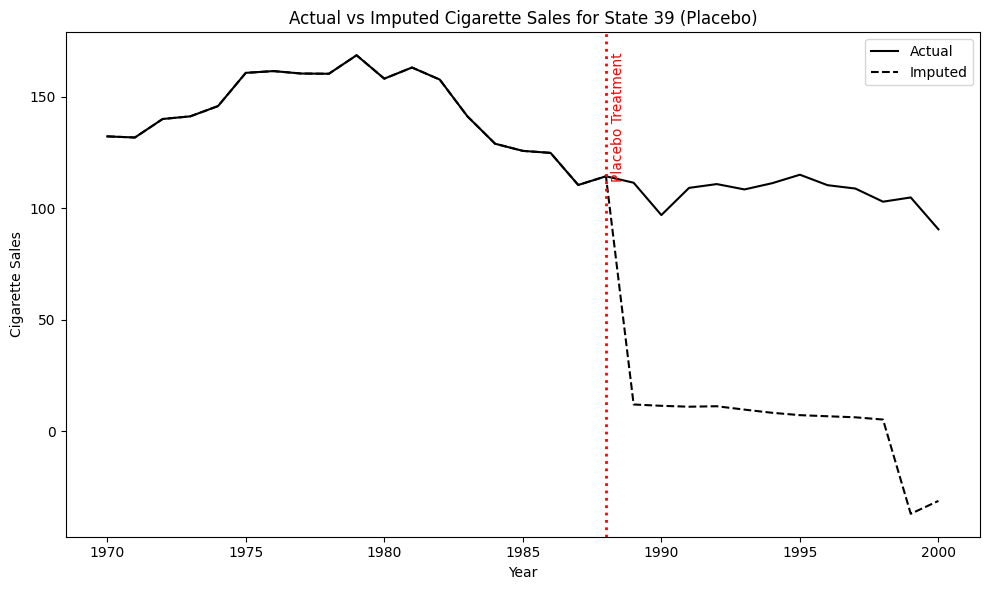
\includegraphics[width=\linewidth]{../figures/cnn_batch_norm-4.png}
        \caption{Wyoming}
        \label{fig:bn-wy}
    \end{subfigure}

    \caption{CNN Counterfactuals with Batch Normalization}
    \label{fig:batch_norm}
\end{figure}

Figure \ref{fig:batch_norm} shows the CNN counterfactuals with batch normalization applied to the California Proposition 99 data.
Panel \ref{fig:bn-cal} shows the counterfactuals for California, the treatment group, and other panels show the counterfactuals for the placebo states (Delaware, Virginia, and Wyoming).

Compared to the original CNN results, the CNN counterfactuals with batch normalization (Figure \ref{fig:batch_norm}) show weaker 
prediction performance. 
Specifically, the counterfactuals plummet after 1989, which is inconsistent in particular with the wide consensus that cigarette sales in California decreased after the implementation of Proposition 99 in 1989.
This suggests that batch normalization may not be suitable for this type of counterfactual prediction task, as the normalization process fits the pre-treatment data too closely, leading to poor generalization to the post-treatment period.


\subsection{Adding Additional Convolutional Layer}

\begin{figure}[htbp]
    \centering
    \begin{subfigure}[b]{0.4\textwidth}
        \centering
        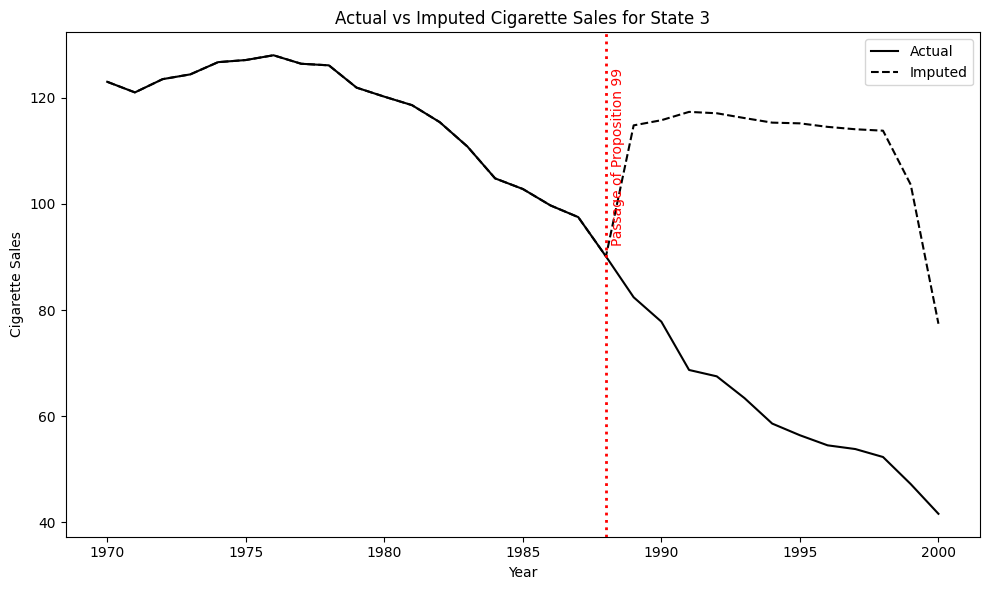
\includegraphics[width=\linewidth]{../figures/cnn_add_layer-1.png}
        \caption{California}
        \label{fig:al-cal}
    \end{subfigure}
    \hspace{1.5cm}
    \begin{subfigure}[b]{0.4\textwidth}
        \centering
        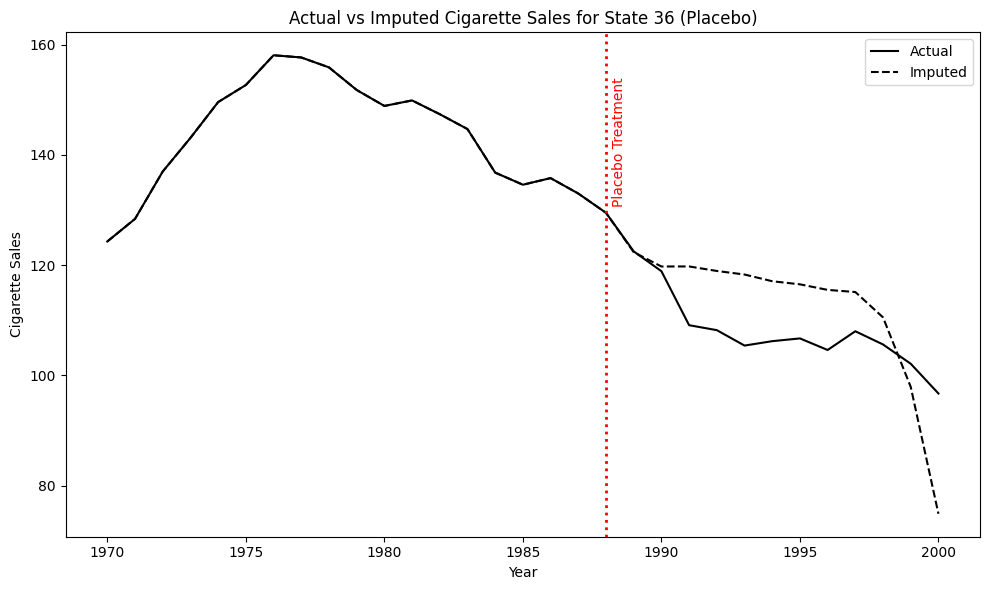
\includegraphics[width=\linewidth]{../figures/cnn_add_layer-2.png}
        \caption{Delaware}
        \label{fig:al-del}
    \end{subfigure}

    \vskip\baselineskip

    \begin{subfigure}[b]{0.4\textwidth}
        \centering
        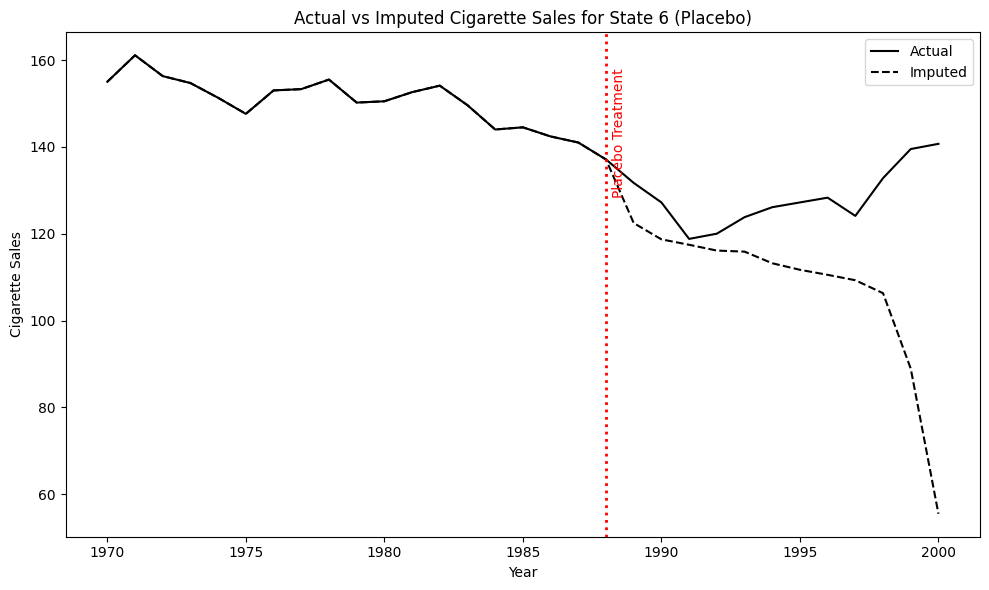
\includegraphics[width=\linewidth]{../figures/cnn_add_layer-3.png}
        \caption{Virginia}
        \label{fig:al-vir}
    \end{subfigure}
    \hspace{1.5cm}
    \begin{subfigure}[b]{0.4\textwidth}
        \centering
        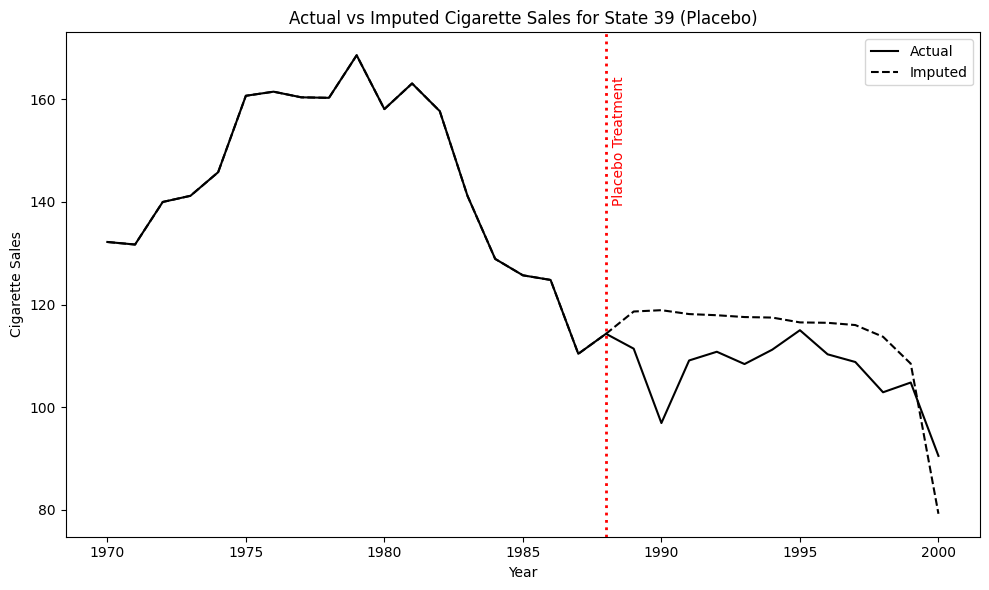
\includegraphics[width=\linewidth]{../figures/cnn_add_layer-4.png}
        \caption{Wyoming}
        \label{fig:al-wy}
    \end{subfigure}

    \caption{CNN Counterfactuals with Additional Layer}
    \label{fig:add_layer}
\end{figure}

Figure \ref{fig:add_layer} shows the CNN counterfactuals with additional convolutional layer with 16 filters and 3$\times 3$ size. applied to the California Proposition 99 data.
Panel \ref{fig:al-cal} shows the counterfactuals for California, the treatment group, and other panels show the counterfactuals for the placebo states (Delaware, Virginia, and Wyoming).

The CNN counterfactuals with additional layer is almost identical to the original CNN results, suggesting that adding an additional convolutional layer does not significantly change the prediction performance.
However, depending on the data size and the complexity of the data generating process, 
adding an additional convolutional layer may improve or worsen the prediction performance in some cases.
